\documentclass[12pt]{article}
\usepackage[utf8x]{inputenc}
\usepackage[colorinlistoftodos]{todonotes}
\usepackage[bookmarks=true]{hyperref}
\usepackage{float}
\usepackage{placeins}
\usepackage{listings}

\begin{document}
	\begin{titlepage}
		\newcommand{\HRule}{\rule{\linewidth}{0.7mm}}
		\center
		
\includegraphics{PolimiLogo.png}\\[1cm]
		
		\textsc{\LARGE Requirements Analysis and Specifications Document}\\[1cm]
		\textsc{\large Software Engineering II Project - A.Y. 2019-2020}\\[1cm]
		\HRule \\[0.4cm]
		{ \huge \bfseries SafeStreets}\\[0.15cm]
		\HRule \\[1.5cm]
		{\large Authors  \hfill ID Numbers}\\[0.4cm]
		{\large Andrea \textsc{Furlan}  \hfill 944774}\\[0.2cm]
		{\large Cosimo \textsc{Russo}  \hfill 945891}\\[0.2cm]
		{\large Giorgio \textsc{Ughini} \hfill 944710}\\[2cm]
		{\large \today  \hfill Version 1.0}
		\vfill
	\end{titlepage}
	\clearpage
	{\hypersetup{hidelinks}\tableofcontents}
	\clearpage
	\section{Introduction}
	\subsection{Purpose}
	The main purpose of SafeStreets is to create a software that provides users the possibility to notify	
authorities	when parking violations occur providing some useful features such as finding the most unsafe areas around them and proposing suggestions to the municipality. In addition, SafeStreets will enable the Local Police to generate traffic tickets from it and to cross all the information it owns with the data of the accidents happened.\\
Specifically, we want to realize a product which is able to:
\begin{itemize}
	
	\item Retrieve pictures uploaded by users of parking violations with possible attached information such as license plate position in the image, type of violation and GPS meta-data.
	
	\item Automatically complete the data of a reported violation running a recognition algorithm able to read license plate text.
	
	\item Highlight to users the areas with the highest frequency of violations and information about vehicles that commit most violations.
	
	\item Automatically identify	potentially unsafe	areas crossing SafeStreets' information with accident datas from the Local Police, possibly	suggesting	possible	interventions.
	
	\item Send violations data to the Local Police to automatically create new traffic tickets if it can be proved that the	chain	of	custody	of	the	information	coming	from	the	users	is	never	broken.
	
	\item Generate statistics related to ticket emissions to inform users about how effective SafeStreets is.
	
\end{itemize}

On the other hand, the purpose of this paper is to define in a detailed way all the functions and requirements of the application.\\ In doing this, we start focusing on a brief overview to characterize the product with relevance to its interaction with the world, then we will proceed deeply in analysing which functions are relevant and should be provided, and which requirements are needed to the stakeholders. 

	\newpage
	\subsubsection{Goals}
	\begin{itemize}

\item \textbf{[\hypertarget{G1}{G1}]} Notifing officers when particular parking violations occur.

\item \textbf{[\hypertarget{G2}{G2}]} Permitting both users and officers to learn which areas have the highest frequency of violations.

\item \textbf{[\hypertarget{G3}{G3}]} Permitting both users and officers to learn which vehicles commit the most violations.

\item \textbf{[\hypertarget{G4}{G4}]} Suggesting possible interventions to potentially unsafe areas.

\item \textbf{[\hypertarget{G5}{G5}]} Allowing the local police to generate automatic traffic tickets from SafeStreets data.

\item \textbf{[\hypertarget{G6}{G6}]} Building and exhibiting statistics.

\end{itemize}
	\vfill
	\subsubsection{Traceability Matrix}
	Since goals, functions and constraints are related to each other a traceability matrix is provided in order to enlight the various relationships among them.
\begin{flushleft}

\begin{table}[htp]
\centering
\begin{tabular}{|l|l|l|l|}
\hline
Goal ID&Functions ID&Constraints ID&UseCases ID\\
\hline
\hyperlink{G1}{G1}&\hyperlink{sec:f1}{F1}&\hyperlink{C1}{C1}, \hyperlink{C3}{C3}, \hyperlink{C4}{C4}, \hyperlink{C6}{C6}&\hyperlink{tab:reportcreationtab}{U1}\\
\hline
\hyperlink{G2}{G2}&\hyperlink{sec:f2}{F2}&\hyperlink{C8}{C8}, \hyperlink{C3}{C3}, \hyperlink{C9}{C9}&\hyperlink{tab:dataminingtab}{U6}, \hyperlink{tab:dataminingofficertab}{U7}\\
\hline
\hyperlink{G3}{G3}&\hyperlink{sec:f3}{F3}&\hyperlink{C3}{C3}, \hyperlink{C7}{C7}, \hyperlink{C8}{C8}&\hyperlink{tab:dataminingofficertab}{U7}\\
\hline
\hyperlink{G4}{G4}&\hyperlink{sec:f4}{F4}&\hyperlink{C2}{C2}, \hyperlink{C4}{C4}, \hyperlink{C6}{C6}&\hyperlink{tab:AutomaticTrafficTicket}{U5}\\
\hline
\hyperlink{G5}{G5}&\hyperlink{sec:f2}{F2}&\hyperlink{C4}{C4}, \hyperlink{C6}{C6}, \hyperlink{C5}{C5}&\hyperlink{tab:dataminingvehicleofficerstab}{U9}, \hyperlink{tab:dataminingvehicletab}{U8}\\
\hline
\hyperlink{G6}{G6}&\hyperlink{sec:f2}{F2}, \hyperlink{sec:f5}{F5}&\hyperlink{C6}{C6}, \hyperlink{C9}{C9}&\hyperlink{tab:statisticsconsultingtab}{U10}\\
\hline
\hyperlink{G7}{G7}&-&-&\hyperlink{tab:statisticsconsultingtab}{U10}\\
\hline
-&\hyperlink{sec:f0}{F0}&-&\hyperlink{tab:signupusecase}{U1}, \hyperlink{tab:loginusecase}{U2}, \hyperlink{tab:recoverpasswordusecase}{U3}\\
\hline

\end{tabular}

\caption{Traceability Matrix} 

\end{table}

\end{flushleft}
	\newpage
	\subsection{Scope}
	As our software needs to be compliant with different laws and as it needs to interact with the Local Police, initially, SafeStreets will have a restricted geographic domain coincident with the Italian
city of Milan. \\
Indeed, in order to provide the most complete service, SafeStreets will require the access the Local Police web application to be able to process traffic tickets. \\
It goes without saying that to organize this kind of service in the most effective way we must experiment first this activity in a internationally-visible city, then applying that to anyone who will demand.
	\subsubsection{The world-machine phenomena}
	\begin{figure}[htp]
	\begin{flushleft}
		The first model of our system to be presented is the model "The world and the machine" by M. Jackson and P. Zave. This model highlights the division between phenomena that happen entirely either in the world or in the machine, and those that are shared between the two of them.
	\end{flushleft}
	\centering
	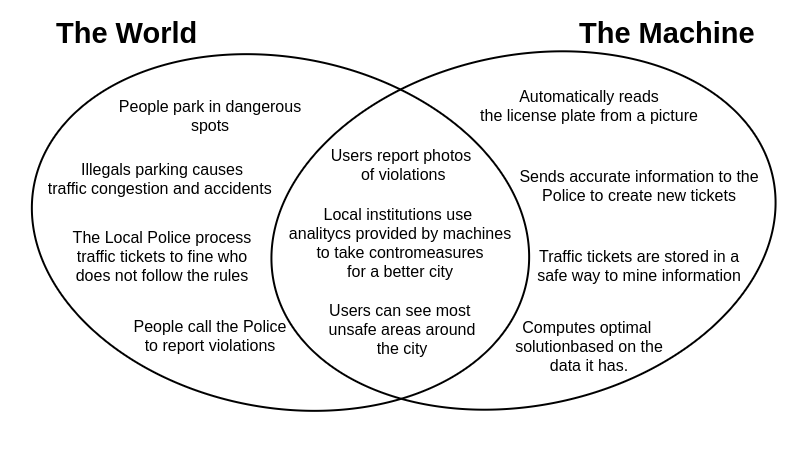
\includegraphics[scale=0.50]{images/world-machine-phenomena}
	\caption{The world-machine phenomena chart.}
	\label{fig:world-machine}
\end{figure}

	\clearpage
	\subsection{Definition and Acronyms}
	\subsubsection{Definitions}
	\begin{itemize}
	\item \textit{Data Mining}: The process of discovering patterns in large data sets involving methods at the intersection of machine learning, statistics, and database systems.
	\item \textit{Computer Vision}: The Computer Vision includes methods for acquiring, processing, analyzing and understanding digital images, to extract high-dimensional data from the real world.
	\item \textit{Report}: The data that a user has provided to the authorities that witness a violation by a vehicles.
	\item \textit{Ticket}: Notice issued by a law enforcement official to a motorist or other road user, indicating that the user has violated traffic laws.
	\item \textit{Violation}: The general infraction that a vehicle has done and that has been reported by a SafeStreets user.
	\item \textit{Guest}: This actor plays the role of a person who is not registered and thus logged in.
	\item \textit{User}: This actor refers to the condition of a normal person (not an officer) already signed up.
	\item \textit{Officer} or \textit{Authority}: This actor represents a public officer that interacts with SafeStreets in some ways.
	\item \textit{Customer}: either a Guest or an Authority
\end{itemize}
	\subsubsection{Acronyms}
	\begin{itemize}
	\item \textbf{AI}:\@ Artificial Intelligence
	\item \textbf{API}:\@ Application Programming Interface
	\item \textbf{CMS}:\@ Content Management System
	\item \textbf{IEEE}:\@ Institute of Electrical and Electronic Engineers
	\item \textbf{GPS}:\@ Global Positioning System
	\item \textbf{OCR}:\@ Optical Character Recognition
	\item \textbf{TLS}:\@ Transport Layer Security
	\item \textbf{UML}:\@ Unified Modeling language
\end{itemize}
	\subsection{References}
	\begin{itemize}
	
	\item The 2019-2020 Software Engineering 2 Project Assignment document
	\item The IEEE Standard for DD
	\item The RASD of SafeStreets
	
\end{itemize}
	\subsection{Document Structure}
	This document is divided in four parts:
\begin{itemize}
	\item \textbf{Introduction}: a description about the goals of SafeStreets and the context in which it will be implemented is provided. A subsection dedicated to the understaing of some acronyms and definitions is also present. 
	
	\item \textbf{Overall Description}: gives an overall description of SafeStreets, focusing on the domain assumptions and the constraints of the application. This section also aims to provide a context to the whole project and to show its integration with the real world. It also shows the possible interactions between the world and the users of SafeStreets. 
	
	\item \textbf{Specific Requirements}: the software requirements, explained in a sufficiently detailed manner to design a system that satisfies them, and the testers to test said requirements are provided.
		
		A detailed description of the possible interactions that can occur between the world and the system is also present, followed by a series of simulations and previews about the interactions mentioned above.
	
	\item \textbf{Formal Analysis using Alloy}: the requirements are expressed through the Alloy model, which, being it is a declarative specification language, makes it possible to define the functions, the constraints and the interactions of SafeStreets.
\end{itemize}
In the last part of the document a short note about the softwares used and the effort spent in producing this RASD by its authors is shown.
	\clearpage
	\section{Overall description}
	\subsection{Product perspective}
	\setlength{\parskip}{1em}
The idea is to create an application to allow users to report parking violations without taking too much time from their daily life.
\\We want therefore to realize an extremely friendly user interface and a lightweight software in order to make SafeStreets affordable to as many people as possible and to be able to run by many devices.

Users will certainly be able to exploit the advanced functions of SafeStreets such as charts and analitycs. However, since those functions rely on data, the basic violations reporting function will be the core one.

Since a small downtime of SafeStreets is not going to cause damage to anyone, it will be tolerated. On the other hand, as our software is going to run some kind of OCR and AI recognition algorithm that will probably be expensive in terms of resources, it should be very dynamic to support different queries in a few seconds.
\\In addition, our software is going to process very specific data that could potentially lead someone to be fined, hence it should ensure that the chain of custody of a report is never broken and the images are never altered.

To upload a new picture on SafeStreets or to view charts about violations, a functional internet connection is required.

The officers appointed to check SafeStreets violations reports will use a system that will access SafeStreets data through its APIs, since a dedicated section for the authorities directly on the app could be exploited by malicious users.

Concerning the hardware, we intend to have a storage system which contains all the historical information about reports made by the users, most likely a database or a data warehouse. This system will allow both users and officers to query for aggregated and detailed information which require a huge amount of data to be processed.
\clearpage
	\subsection{Class Diagram}
	\begin{figure}[htp]
	\centering
	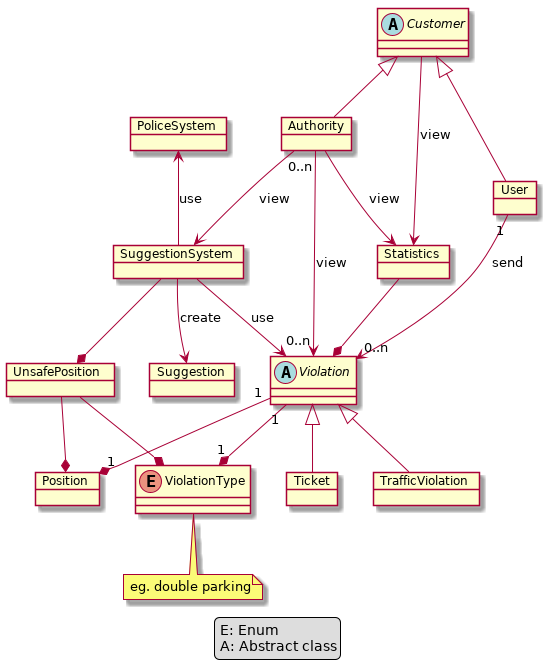
\includegraphics[width=\textwidth]{images/Class Diagram.png}
	\caption{The class diagram of SafeStreets.}
	\label{fig:class-diagram}
\end{figure}

	\subsection{Product functionalities}
	This section provides an abstract of the main functions of the application. To be able to use any of the given functionalities, the user must first register and then login to the application by providing a valid email and a password.
\subsubsection[Notification of Violations]{[F1] Notification of Violations\hypertarget{sec:f1}{}}
\label{sec:notification_of_violations}
The base function of the application is the possibility to signal a traffic violation.

The user must send one or more picture(s) of the car in which both the violation and the license plate are clearly visible.

The application will try to automatically get the user position using its GPS system, and will notify the user in case of failure so that it can enter it manually.

The users will then send the following information to the system:
\begin{itemize}
    \item The pictures selected by the user
    \item The position of the user
    \item The current date and time
    \item The type of violation (to be picked from a pre-defined list)
    \item An optional comment inserted by the user
\end{itemize}
The information sent by the user will be stored on persistent storage on the server and the officers will be able to see it on their clients.

\subsubsection[Data Mining]{[F2] Data Mining\hypertarget{sec:f2}{}}
The system will allow both users and officers to extract statistics about violations in the various areas/streets of the cities in the system,
for example a user can find the areas in which most reports occurred in the last 3 months.

Data mining must take into account the privacy of the users.
To guarantee an acceptable level of privacy, different roles are given to the users and the officers.

In particular, a user will only be able to see statistics provided by aggregated data, never he will see the absolute numbers but only percentages. 

Officers will, instead, have the finest granularity: they will see all the information enriched by the actual number of violations and can drill down to the specific licence plates which committed the violations.
They will also have more filters available with respect to the users, for example the possibility to see which cars committed most violations in a given period.

\subsubsection[Request for interventions]{[F3] Request for interventions\hypertarget{sec:f3}{}}
\label{sec:request_for_interventions}
The system will get information from the local police systems about incidents, including the location, the licence plates of the cars involved, and the infractions committed.

By crossing the data about the incidents with the segnalations from its users, SafeStreets will be able to find unsafe areas and also to suppose a reason for it and make suggestions.
For example, if a road has many cyclists hit and many signals of cars parked on the bike lane, it can suggest to add a barrier between the parking lane and the road.
The correlations between the infractions found on the police system and the ones on the SafeStreet system, along with the possible solutions, will be done automatically and can be revised by hand by a officer.
An artificial intelligence can then help to calibrate when the system should launch a warning, training on the approval/rejection of the previous signals.

The officers responsible for handling these recommendations will see on their clients all the data about the signal,
including the number of incidents and signals, and can decide to discard it or approve it, thus keeping it in the system for future reference.
All the approved signals will be reachable by the officers, once they have been resolved they can be deleted from the list but will remain in an archive available for the AI.


\subsubsection[Automatic Tickets]{[F4] Automatic Tickets\hypertarget{sec:f4}{}}
\label{sec:automatic_tickets}
The user will be indirectly able to give tickets when he spots a violation. This works by adding to the functionality
\hyperref[sec:notification_of_violations]{"Notification of Violations"}
the possibility to confirm that he is sure that he is signalling an actual violation and wants to give a ticket.
In this case the system reads the licence plate and uses the police system to automatically issue a ticket.

Security is a key aspect of this functionality. The system must be sure that the signal has not been modified.
To achieve this, all messages are encrypted with TLS and an hash of every picture is included in the message.

\subsubsection[Statistics]{[F5] Statistics\hypertarget{sec:f5}{}}
The system will also be able to build statistics using the violation and ticket systems.
These data will represent the amount of tickets given in a certain street/area in a given period, the most egregious offenders, and the change in the number of tickets in a certain place during time.
Just like in the
\hyperlink{sec:f2}{Data Mining}
section, users will not be able to obtain information on single people, they will only see aggregated data and percentages instead of total numbers.
The officers will instead have the possibility to see the actual numbers and to get information about specific license plates.
\clearpage
	\subsubsection{Traceability Matrix}
	Since goals, functions and constraints are related to each other a traceability matrix is provided in order to enlight the various relationships among them.
\begin{flushleft}

\begin{table}[htp]
\centering
\begin{tabular}{|l|l|l|l|}
\hline
Goal ID&Functions ID&Constraints ID&UseCases ID\\
\hline
\hyperlink{G1}{G1}&\hyperlink{sec:f1}{F1}&\hyperlink{C1}{C1}, \hyperlink{C3}{C3}, \hyperlink{C4}{C4}, \hyperlink{C6}{C6}&\hyperlink{tab:reportcreationtab}{U1}\\
\hline
\hyperlink{G2}{G2}&\hyperlink{sec:f2}{F2}&\hyperlink{C8}{C8}, \hyperlink{C3}{C3}, \hyperlink{C9}{C9}&\hyperlink{tab:dataminingtab}{U6}, \hyperlink{tab:dataminingofficertab}{U7}\\
\hline
\hyperlink{G3}{G3}&\hyperlink{sec:f3}{F3}&\hyperlink{C3}{C3}, \hyperlink{C7}{C7}, \hyperlink{C8}{C8}&\hyperlink{tab:dataminingofficertab}{U7}\\
\hline
\hyperlink{G4}{G4}&\hyperlink{sec:f4}{F4}&\hyperlink{C2}{C2}, \hyperlink{C4}{C4}, \hyperlink{C6}{C6}&\hyperlink{tab:AutomaticTrafficTicket}{U5}\\
\hline
\hyperlink{G5}{G5}&\hyperlink{sec:f2}{F2}&\hyperlink{C4}{C4}, \hyperlink{C6}{C6}, \hyperlink{C5}{C5}&\hyperlink{tab:dataminingvehicleofficerstab}{U9}, \hyperlink{tab:dataminingvehicletab}{U8}\\
\hline
\hyperlink{G6}{G6}&\hyperlink{sec:f2}{F2}, \hyperlink{sec:f5}{F5}&\hyperlink{C6}{C6}, \hyperlink{C9}{C9}&\hyperlink{tab:statisticsconsultingtab}{U10}\\
\hline
\hyperlink{G7}{G7}&-&-&\hyperlink{tab:statisticsconsultingtab}{U10}\\
\hline
-&\hyperlink{sec:f0}{F0}&-&\hyperlink{tab:signupusecase}{U1}, \hyperlink{tab:loginusecase}{U2}, \hyperlink{tab:recoverpasswordusecase}{U3}\\
\hline

\end{tabular}

\caption{Traceability Matrix} 

\end{table}

\end{flushleft}
	\subsection{User characteristics}
	The users of SafeStreets can be both males or females of any age with no particular limitations. Of course, said users should have at least a basic knowledge of smartphones and electronic devices in general, especially on how to make photos and videos.
Users should also have an e-mail address, primarily used to register and authenticate themselves.\\
Officers instead can also be both males or females but they need to be actual public officers enrolled in the Local Police.
They should have a medium knowledge of networks, softwares and hardwares as well as a fully understanding of how traffic tickets laws can be applied, and they should be capable of using municipality tools and softwares fluently.
	
	\subsection{Assumptions and dependencies}
	\subsubsection{Domain Assumptions}
	\begin{itemize}

\item A user should input only correct data when reporting a violation, for example the license plate position on the picture(s) shot should be correct

\item The image and picture meta-data aren't altered by the user who first submits the report

\item The municipality will provide provide correct and complete information 
about the accidents

\item The municipality services will not be offline for more than 5 minutes in a row during the uptime of SafeStreet
\item A report sent by a user must be taken in consideration by an officer in a reasonable time.

\end{itemize}
	
	\subsubsection{General Assumptions}
	\begin{itemize}
    \item A user cannot access any of the functionality of the application if he does not register first.
        The registration approach will be similar to the one used by social media: the user will provide his first and last name, hit birthday, an email, a password and a profile picture.
        All these data will be automatically approved during the registration phase, and the user will be able to use the SafeStreets functions right away.
        a user can be banned at any time if it uses the application in a non-compliant way, for example if he sends a fake violation report.
    \item Since users could be accountable for what they do with the app (they could be banned), we suppose that they will use SafeStreets
        in the most responsible way. For this reason, all tickets that are inserted correctly will be automatically approved.
\end{itemize}
	\clearpage
	\subsubsection{Constraints}
	\begin{itemize}
	\item \textbf{[\hypertarget{C1}{C1}]} It is impossible to send a report without attaching a picture, a description and selecting a reason that represents the violation. 
	\item \textbf{[\hypertarget{C2}{C2}]} It is impossible to cancel an already sent ticket. 
	\item \textbf{[\hypertarget{C3}{C3}]} It is prevented to attach a non-valid address to a report.
	\item \textbf{[\hypertarget{C4}{C4}]} It is prevented to send a report with a picture that contains non-readable license plate. 
	\item \textbf{[\hypertarget{C5}{C5}]} Searching the license plate of a person in the worst driver section is forbidden.
	\item \textbf{[\hypertarget{C6}{C6}]} Giving multiple tickets to the same car for a single violation is prevented
	\item \textbf{[\hypertarget{C7}{C7}]} A suggestion for a possible intervention is destined to the authorities only.
	\item \textbf{[\hypertarget{C8}{C8}]} An unsafe area is determined as such if it has received a consistent amount of certified violations (from SafeStreets) and accidents (from the police service) in the last month. 
	\item \textbf{[\hypertarget{C9}{C9}]} Statistics are generated using all and only the succesfully submitted reports.
	\item \textbf{[\hypertarget{C10}{C10}]} The issue of reports which location is outside the competence area of the local police is prevented
	
	%%%
	%%% Forse queste potremmo chiedere al prof se tenerle o meno?
	%%%
	%%%\item \textbf{[\hypertarget{C1}{C1}]} It is impossible to login without being signed up. 
	%%%\item \textbf{[\hypertarget{C2}{C2}]} Is impossible to login if already logged in. 
	%%%\item \textbf{[\hypertarget{C3}{C3}]} Is impossible to signup if already signed up.
	%%%\item \textbf{[\hypertarget{C9}{C9}]} The chain of custody of the information coming from the users shouldn't be broken.
	%%%
\end{itemize}
\clearpage

	\subsubsection{Traceability Matrix}
	Since goals, functions and constraints are related to each other a traceability matrix is provided in order to enlight the various relationships among them.
\begin{flushleft}

\begin{table}[htp]
\centering
\begin{tabular}{|l|l|l|l|}
\hline
Goal ID&Functions ID&Constraints ID&UseCases ID\\
\hline
\hyperlink{G1}{G1}&\hyperlink{sec:f1}{F1}&\hyperlink{C1}{C1}, \hyperlink{C3}{C3}, \hyperlink{C4}{C4}, \hyperlink{C6}{C6}&\hyperlink{tab:reportcreationtab}{U1}\\
\hline
\hyperlink{G2}{G2}&\hyperlink{sec:f2}{F2}&\hyperlink{C8}{C8}, \hyperlink{C3}{C3}, \hyperlink{C9}{C9}&\hyperlink{tab:dataminingtab}{U6}, \hyperlink{tab:dataminingofficertab}{U7}\\
\hline
\hyperlink{G3}{G3}&\hyperlink{sec:f3}{F3}&\hyperlink{C3}{C3}, \hyperlink{C7}{C7}, \hyperlink{C8}{C8}&\hyperlink{tab:dataminingofficertab}{U7}\\
\hline
\hyperlink{G4}{G4}&\hyperlink{sec:f4}{F4}&\hyperlink{C2}{C2}, \hyperlink{C4}{C4}, \hyperlink{C6}{C6}&\hyperlink{tab:AutomaticTrafficTicket}{U5}\\
\hline
\hyperlink{G5}{G5}&\hyperlink{sec:f2}{F2}&\hyperlink{C4}{C4}, \hyperlink{C6}{C6}, \hyperlink{C5}{C5}&\hyperlink{tab:dataminingvehicleofficerstab}{U9}, \hyperlink{tab:dataminingvehicletab}{U8}\\
\hline
\hyperlink{G6}{G6}&\hyperlink{sec:f2}{F2}, \hyperlink{sec:f5}{F5}&\hyperlink{C6}{C6}, \hyperlink{C9}{C9}&\hyperlink{tab:statisticsconsultingtab}{U10}\\
\hline
\hyperlink{G7}{G7}&-&-&\hyperlink{tab:statisticsconsultingtab}{U10}\\
\hline
-&\hyperlink{sec:f0}{F0}&-&\hyperlink{tab:signupusecase}{U1}, \hyperlink{tab:loginusecase}{U2}, \hyperlink{tab:recoverpasswordusecase}{U3}\\
\hline

\end{tabular}

\caption{Traceability Matrix} 

\end{table}

\end{flushleft}
	
	\clearpage
	\section{Specific requirements}
	\subsection{External Interface Requirements}
	\subsubsection{User Interfaces}
	Concerning the user interface requirements, a series of mockups that represent how the application layout should be is provided. Changes that won't alter SafeStreets functioning can be applied during the implementation.\\
The sketches of the main pages of SafeStreets are designed with the aim to make the application as user friendly as possible since many "inexperienced" people (like 60s years old) could be the principal users. Still, since the following mockups are more concepts than rules, the design could take a more technical path. \\

	\subsubsection{Software Interfaces}
	Considering the domain of our application, we  decided to integrate in our project some software components to create an easier-to-use product. 
\\In order to provide users the ability to automatically insert location info into their violation pictures meta-data, we chose to adopt a location provider service. That supplier should expose an API to retrieve the user exact address by his or her GPS position coordinates. 
\\In addition, APIs provided by the municipality are required to retrieve real time information about the accidents	that	occurred	on	the	territory	of	the	municipality to allow information mining and suggestion proposing.
\\Finally, the Local Police is required to provide an API to retrieve information about violation coming from SafeStreets users to create and process traffic ticket from it.
	\begin{figure}
	\begin{flushleft}
		\textbf{Login Page}:\\
		Since logging into SafeStreets is mandatory, this is the first page that the user will face when the app does not recognizes him. Of course, cookies or sessions could avoid to force the user to login every time.
	\end{flushleft}
	\centering
	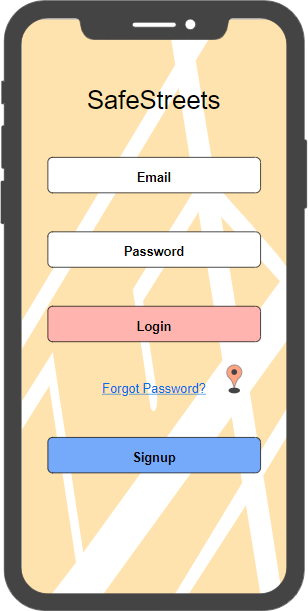
\includegraphics[width=0.6\linewidth]{../RASD/images/mockups/login}
	\caption{SafeStreets Login page.}
\label{fig:login}
\end{figure}
\clearpage
\begin{figure}
	\begin{flushleft}
		\textbf{SignUp Page}:\\
		Since logging into SafeStreets is mandatory, if the user does not have an account he needs to make one. Every field except the photo should be mandatory.
	\end{flushleft}
	\centering
	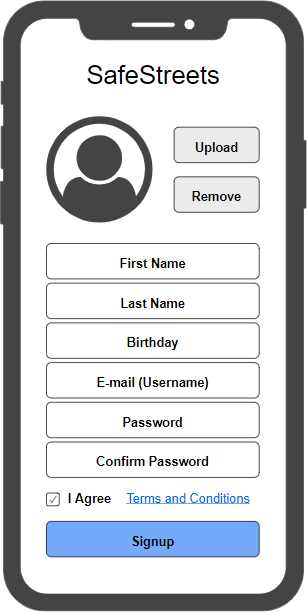
\includegraphics[width=0.6\linewidth]{../RASD/images/mockups/signup}
	\caption{SafeStreets SignUp page.}
	\label{fig:signup}
\end{figure}
\clearpage
\begin{figure}
	\begin{flushleft}
		\textbf{Home Page}:\\
		When the user logs into SafeStreets successfully, an home page should be provided with the options for the user to use every functionality of the application.
	\end{flushleft}
	\centering
	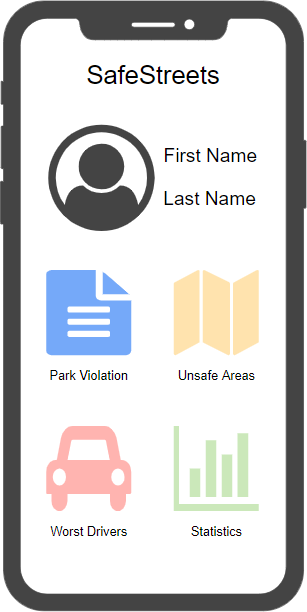
\includegraphics[width=0.6\linewidth]{../RASD/images/mockups/homePage}
	\caption{SafeStreets Home page.}
	\label{fig:home}
\end{figure}
\clearpage
\begin{figure}
	\begin{flushleft}
		\textbf{Violation Page}:\\
		If the user wants to send to the officers a parking violation of some sorts a form to be filled is provided. The user can either send a report that will generate an automatic ticket or that will need to be checked by the officers.
	\end{flushleft}
	\centering
	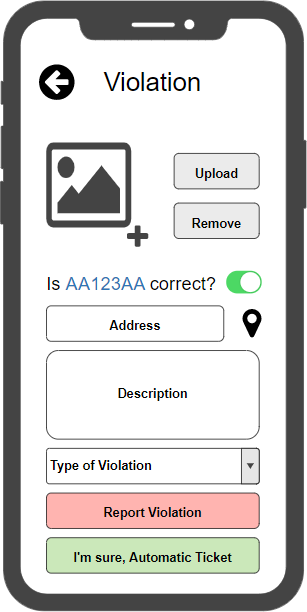
\includegraphics[width=0.6\linewidth]{../RASD/images/mockups/violation}
	\caption{SafeStreets Violation page.}
	\label{fig:violation}
\end{figure}
\clearpage
\begin{figure}
	\begin{flushleft}
		\textbf{Unsafe Areas Page}:\\
		If the user wants to see which areas are the most subject to violations, an interface to search among all areas should be implemented.
	\end{flushleft}
	\centering
	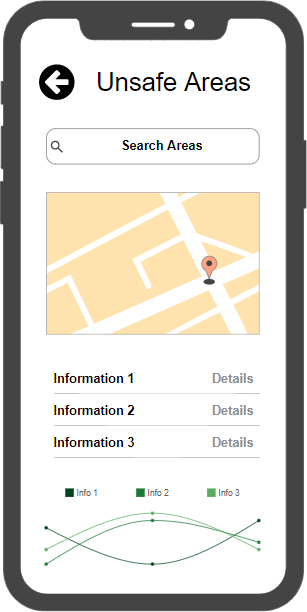
\includegraphics[width=0.6\linewidth]{../RASD/images/mockups/areas}
	\caption{SafeStreets Unsafe Areas page.}
	\label{fig:areas}
\end{figure}
\clearpage
\begin{figure}
	\begin{flushleft}
		\textbf{Worst Drivers Page}:\\
		If the user wants to see which vehicles tends to not follow the city rules, an interface that shows this needs to be present in the application.
	\end{flushleft}
	\centering
	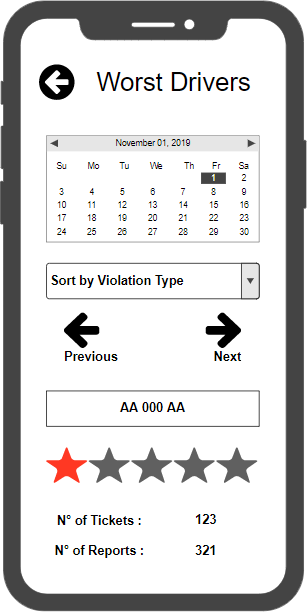
\includegraphics[width=0.6\linewidth]{../RASD/images/mockups/vehicles}
	\caption{SafeStreets Worst Drivers page.}
	\label{fig:vehicles}
\end{figure}
\clearpage
\begin{figure}
	\begin{flushleft}
		\textbf{Statistics Page}:\\
		A complete page that exhibits all of SafeStreets data in a complete and detailed manner, that also enlightens SafeStreets effectiveness. 
	\end{flushleft}
	\centering
	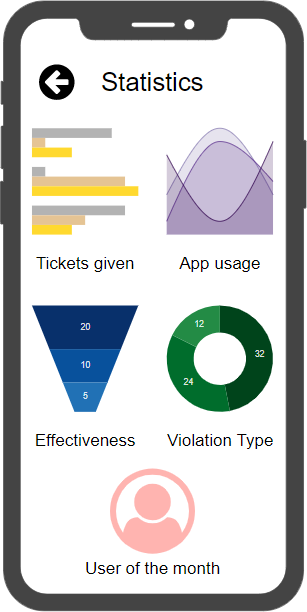
\includegraphics[width=0.6\linewidth]{../RASD/images/mockups/statistics}
	\caption{SafeStreets Statistics page.}
	\label{fig:statistics}
\end{figure}
\clearpage
\begin{figure}
	\begin{flushleft}
		\textbf{User Profile Page}:\\
		If the user wants to change its profile picture or his password, if he wants to check his reports or to logout, he should be able to do all these things. 
	\end{flushleft}
	\centering
	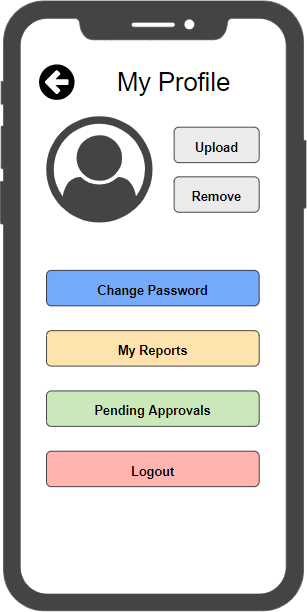
\includegraphics[width=0.6\linewidth]{../RASD/images/mockups/profile}
	\caption{SafeStreets User Profile page.}
	\label{fig:profile}
\end{figure}
\clearpage
	\clearpage
	\subsection{Scenarios}
	\subsubsection{First scenario}
	\begin{table}[!htbp]
\begin{tabular}{lp{9.5cm}}
\hline
\bf\large  &\bf\large Creation of a report\\
\hline
\hline

\bf Actors&Mario Rossi and Luca Neri: habitual users\\
\bf &Maurizio Verdi: a car owner\\
\hline
\bf Flow of events&
Maurizio is driving his car to reach his girlfriend house. Once arrived, he leaves his car double parked because he don't want to spend much time looking for a park.
Mario is - as always - taking his dog out before dinner and is directed trough the park situated five minute by food. While walking, he notices that Maurizio's car is double parked and is slowing down all the cars running in the street. His dog is making more than an effort to go to the park and so Mario wouldn't have much time to call the Police to report this violation.
Meanwhile, Luca is - as always - getting back home by car. He lives outside the city and he thinks the train is not trustworthy so he chose the car. But getting out of the city at 7PM is always very slow because of the many dribbling the cars should do to avoid other cars parked on the lane and that said, he's late for the dinner with his wife.  
Mario, still in a hurry, takes out his mobile phone and opens SafeStreets app. From the homepage he create a new report and the process didn't take much time: only what is required to shoot a photo and select the double park infraction from the menu. So, after a few seconds, he was again able to walk with his dog trough the park. That day, Luca ended up arriving late at home and eating alone his cold meal. As soon as Maurizio receives the ticket from the Local Police he realize that, now that the world has SafeStreets, it's worth the time to seek a legal parking to avoid being fined again. As days go by, more car owner realize the same thing and all this ends up in Luca being able to come back home with less pain after his long days of work.\\
\end{tabular}
\caption{Scenario 1} 
\label{tab:scenarioone}
\end{table}
	\FloatBarrier
	\subsubsection{Second scenario}
	\begin{table}[!htbp]
	\centering
\begin{tabular}{lp{9.5cm}}
\hline
\bf\large  &\bf\large Data mining and suggestion proposal\\
\hline
\hline

\bf Actors&Giovanni Ciano: head officer of the Local Police\\
\hline
\bf Flow of events&
As situations like double parking keeps happening in the same area as in \autoref{tab:scenarioone}, many car owner are getting more polite and respectful, but it is still not enough. Indeed, one day, Giovanni receives a letter from the mayor asking him to find a way to help solving the city mobility problem in that area. It is a difficult problem to handle by his own and he does not have enough data and suggestions from his officers because it seems that they cannot find a pattern. Giovanni is desperate but then he has an idea: he opens his SafeStreets control panel and sees that there are suggestions not examined yet. The software has detected that the same double parking violation keeps occurring and it therefore alerts Giovanni to proceed with the automatic detection of parking infractions.
The automatic detection of such infraction is a mechanism, adopted by the Local Police, that consists in putting a special video camera on a Police car and then driving along the streets to automatically fine all car owners that are not compliant with the local laws. Giovanni schedules it for the next Friday: two officers will take care of it. After that raid, fifteen different parking violations were discovered all in the same street! Without SafeStreets, Giovanni wouldn't have ever imagined that such a disease was taking place in that street, but thanks to the suggestion he received, now car owners will certainly respect the law, avoiding slowing down the traffic in that street.
\end{tabular}
\caption{Scenario 2} 
\label{tab:scenariotwo}
\end{table}
	\FloatBarrier
	\clearpage
	\subsubsection{Third scenario}
	\begin{table}[!htbp]
	\centering
\begin{tabular}{lp{9cm}}
\hline
\bf\large  &\bf\large Data mining and suggestion proposal\\
\hline
\hline

\bf Actors&Matteo Neri: officer of the Local Police\\
\hline
\bf Flow of events&
Summer is a great season, there are less workers and students in the city and many of them use bikes or go to work by foot.
Every autumn, instead, people in the city begin to leave their bike at home and head to work by car. Matteo is perfectly aware of this situation because, as usual, on October his head officer sends him and his colleagues to a few intensive sessions of heavy fining to car parked in the wrong way. Matteo thinks he could do more for the city than fining people all day, and is always bored by it. Ever since when SafeStreets has been introduced, citizens and normal users have become impressive reporter of violations and this behaviour keeps growing. Having realized this, now Matteo and his colleagues can be assigned to more meaningful tasks, for example they could handle the traffic near the schools when it starts or ends. Matteo is now more happy of working and he thinks he's contributing to his city in a better way, improving the kids and their parents quality of life.
\end{tabular}
\caption{Scenario 3} 
\label{tab:scenariothree}
\end{table}
	\FloatBarrier
	\clearpage
	\subsection{Functional Requirements}
	\newcommand{\usecasefigure}[2]{
	\begin{figure}[htp]
		\centering
		\includegraphics[width=1.0\textwidth]{images/useCases/#1.png}
		\caption{Use case diagram #2}
		\label{fig:use_cases_#1}
	\end{figure}
	\newpage
}

\newcommand{\usecasefiguresmall}[2]{
	\begin{figure}[htp]
		\centering
		\includegraphics[width=0.95\textwidth]{images/useCases/#1.png}
		\caption{Use case diagram #2}
		\label{fig:use_cases_#1}
	\end{figure}
	\newpage
}

\newcommand{\usecasefiguresmaller}[2]{
	\begin{figure}[htp]
		\centering
		\includegraphics[width=0.85\textwidth]{images/useCases/#1.png}
		\caption{Use case diagram #2}
		\label{fig:use_cases_#1}
	\end{figure}
	\newpage
}

This section contains all the use cases initially described with the use case UML models, then the most important Use Cases have their own table which provides further details such as: involved actors, entry conditions, flow of events,  exit conditions and exceptional conditions.

\subsubsection{User Page use cases}
\begin{figure}[htp]
	\centering
	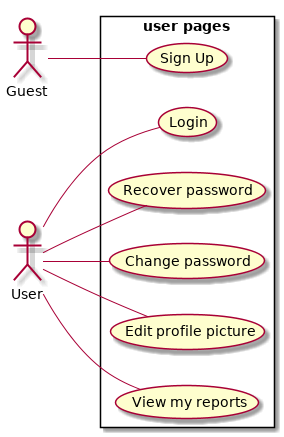
\includegraphics[width=0.6\textwidth]{images/useCases/uc_user_page.png}
	\caption{Use cases relative to the user registration and authentication} 
	\label{fig:userpage} 
\end{figure} 

\newpage
\begin{enumerate}
	\item \textbf{Sign Up}\\
		\begin{table}[!htbp]
\centering
\begin{tabular}{lp{8cm}}
\bf\large Name&\bf\large Sign up\\
\hline
\hline
\bf Actors&Guest\\
\hline
\bf Entry conditions&None\\
\hline
\bf Flow of events&
\begin{itemize}
\item The guest reaches the registration page containing the relative form
\item The guest fills up the form and clicks on "Sign up" to complete the process
\item The system redirects the user to his profile page.
\end{itemize}
\\
\hline
\bf Exit conditions&The guest has successfully registered into SafeStreets. \\
\hline
\bf Exceptions&The guest left an empty field or typed
 something invalid: an error message is displayed 
 and the user is asked to fill the form again.\\
\hline

\end{tabular}
\caption{Use Case table - Sign up} \label{tab:signup}
\end{table}

		\newpage
		\textbf{Diagrams}
		\usecasefigure{sign_up}{of the signup process}
		\newpage
	\item \textbf{Login}\\
		\begin{table}[!htbp]
\centering
\begin{tabular}{lp{8cm}}
\bf\large Name&\bf\large Login\\
\hline
\hline
\bf Actors&User\\
\hline
\bf Entry conditions&The user had already registered in the past.\\
\hline
\bf Flow of events&
\begin{itemize}
\item The user reaches the login page containing the relative form
\item The user types the username and password in the login form and clicks on the "Login" button.
\item The system redirects the user to the application homepage.
\end{itemize}
\\
\hline
\bf Exit conditions&The user has access to the application functionalities. \\
\hline
\bf Exceptions&Username and password didn't correspond or the username didn't exist: an error message is displayed and the user is asked to fill the login form again.\\
\hline

\end{tabular}

\caption{Login Use Case table} \label{tab:login}
\end{table}
		\newpage
		\textbf{Diagrams}
		\usecasefigure{login}{of the login process}
		\newpage
	\item \textbf{Password Recovery}\\
		\begin{table}[!htbp]
	
	\hypertarget{tab:recoverpasswordusecase}{}
	\centering
	\begin{tabular}{lp{8cm}}
		\bf\large Name&\bf\large Recover Password \\
		\hline
		\hline
		\bf Actors&User\\
		\hline
		\bf Entry conditions&The user had already registered in the past.\\
		\hline
		\bf Flow of events&
		\begin{itemize}
			\item The user reaches the login page containing the relative form
			\item The user does not remember his password so he clicks on "Password recovery" button and is redirected to the password recovery page.
			\item The user inserts his email and clicks on "reset password".
			\item The system sends an email to the user with a link and instruction to reset the password.
			\item The user chooses and types a new password and confirms.
			\item The system redirects the user to the login page.
		\end{itemize}
		\\
		\hline
		\bf Exit conditions&The user requested an email to reset his password \\
		\hline
		\bf Exceptions&The inserted email does not match any user in the database, it is displayed an error message and the user is asked to retype a valid email.\\
		\hline
		
	\end{tabular}
	\caption{Recover password Use Case table} \label{tab:recoverpassword}
\end{table}
		\newpage
		\textbf{Diagrams}
		\usecasefiguresmall{password_recovery}{of the password recovery process}
		\newpage
\end{enumerate}
\newpage

\subsubsection{Report and Information Management use cases}
\begin{figure}[htp]
	\centering
	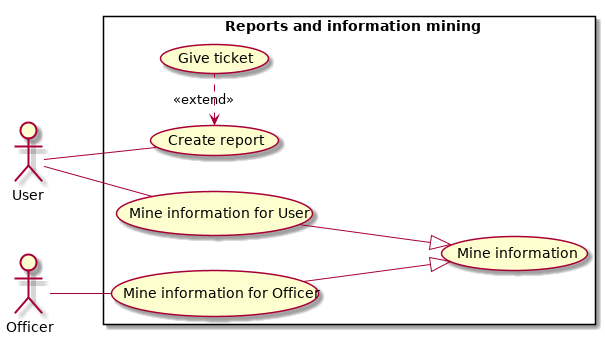
\includegraphics[width=\textwidth]{images/useCases/uc_report_and_information_mining.png}
	\caption{Main use cases showing the functionalities of SafeStreets application relative to the user report management and information mining.} 
	\label{fig:reportmanagement} 
\end{figure}

\newpage
\begin{enumerate}
	\setcounter{enumi}{3}
	\item \textbf{Report Creation}\\
		\begin{table}[!htbp]
	\centering
	\begin{tabular}{lp{9cm}}
\bf\large Name&\bf\large Creation of a new report\\
\hline
\hline
\bf Actors&User\\
\hline
\bf Entry conditions&The user is logged in and is in the main page.\\
\hline
\bf Flow of events&
\begin{itemize}

\item The user clicks on "Report Violation" button and is redirected to the page with the input form to create a new report.

\item The user fills up the form with the violation information (type of violation, pictures of it, address, description, license plate position, date and time, etc...). Eventually some fields such as date and time will be auto-completed.

\item The user clicks on the "Send Report" button after a quick check of all the field he typed.

\item The system show the user a confirmation message. 

\item The user is then redirected to the main page.

\end{itemize}
\\
\hline
\bf Exit conditions&The new report with the user-inserted data is created into the SafeStreets system. In the case of the violation to result in a duplicate (possibly by another user) of in case of the license plate to be not readable, the system put this report in a revision queue and block the process.\\
\hline
\bf Exceptions&The information inserted is wrong (non-existent address, date and time in the future) or some information is missing: a corresponding error is displayed and the user is asked to modify the inserted information accordingly.
\\
\hline

\end{tabular}
\caption{Report Creation Use Case table}
 \label{tab:reportcreationtab}
\end{table}
		\newpage
		\textbf{Diagrams}
		\usecasefigure{creation_of_new_report}{of the report creation process}
		\newpage
	\item \textbf{Automatic Traffic Ticket generation}\\
		\begin{table}[!htbp]
	\hypertarget{tab:AutomaticTrafficTicket}{}
	\centering
	\begin{tabular}{lp{10cm}}
\bf\large Name&\bf\large Automatic Traffic Ticket generation\\
\hline
\hline
\bf Actors&User\\
\hline
\bf Entry conditions&The user is logged in and is in the main page.\\
\hline
\bf Flow of events&
\begin{itemize}
\itemsep0em 
\item The user clicks on "Report Violation" button and is redirected to the input form to create a report.

\item The user fills up the form with the violation information (type of violation, pictures of it, address, description, license plate position, date and time, etc...). Eventually some fields such as date and time will be auto-completed.

\item The user clicks on the "Verified Violation" checkbox because he is sure of it being a violation because it's evident or any other motivation.

\item The user clicks on the "Send Report" button after a quick check of all the field he typed.

\item The system shows a confirmation message to the user and redirects him to the main page.

\end{itemize}
\\
\hline
\bf Exit conditions&The new report is created into the SafeStreets system and passed to the Local Police service.\\
\hline
\bf Exceptions&
\setlist{nolistsep}
\begin{itemize}
	\itemsep0em 
	\item The information inserted is wrong (non-existent address, date and time in the future) or some information is missing: a corresponding error is displayed and the user is asked to modify the inserted information accordingly.
	\item The violation results in a duplicate or the license plate is not readable: the system put this report in a revision queue and block the process.
\end{itemize}
\\
\hline

\end{tabular}
\caption{Automatic Traffic Ticket generation Use Case table}
 \label{tab:AutomaticTrafficTicket}
\end{table}
		\newpage
		\textbf{Diagrams}
		\usecasefigure{automatic_traffic_ticket}{of the traffic ticket generation process}
		\newpage
	\item \textbf{Information Mining by Users (Unsafe Area)}\\
		\begin{table}[!htbp]
	\hypertarget{tab:dataminingtab}{}
	\centering
	\begin{tabular}{lp{9cm}}
\bf\large Name&\bf\large Information Mining by users\\
\hline
\hline
\bf Actors&User\\
\hline
\bf Entry conditions&The user is logged in and is in the main page.\\
\hline
\bf Flow of events&
\begin{itemize}

\item The user clicks on the "Unsafe Areas" button and is redirected to the page with the general SafeStreets statistics about various areas in the city.

\item The user clicks on the selection menu to choose which area he wants to see, possibly entering its name or an address in that area.

\item The user could analyze the data that will be shown with a practical map and the textual information.

\item After he finishes, he presses the Home button.

\item The user is then redirected to the main page.

\end{itemize}
\\
\hline
\bf Exit conditions&The user-requested analytics is displayed to the user at the level of aggregation he has chosen (these kind of information is not sensitive).\\
\hline
\bf Exceptions&The selected area is actually not present on SafeStreets or nonexistent: an error is displayed and he is asked to modify the inserted location accordingly.
\\
\hline

\end{tabular}
\caption{Data Mining Use Case table}
 \label{tab:dataminingtab}
\end{table}
		\newpage
		\textbf{Diagrams}
		\usecasefiguresmaller{information_mining}{of the information mining process (unsafe area) for a user}
		\newpage
	\item \textbf{Information Mining by Officers (Unsafe Area)}\\
		\begin{table}[!htbp]
	\hypertarget{tab:dataminingofficertab}{}
	\centering
	\begin{tabular}{lp{9cm}}
\bf\large Name&\bf\large Information Mining by officers\\
\hline
\hline
\bf Actors&Officer\\
\hline
\bf Entry conditions&The officer is logged in and is in the main page of his software.\\
\hline
\bf Flow of events&
\begin{itemize}

\item The officer clicks on the "Statistics" section button and is redirected to a page with the general SafeStreets statistics (such as number of usages, last use date, etc) in the officer municipality.

\item The officer clicks on the selection menu to switch between statistics related to his municipality, possibly exporting it in CSV (most dangerous areas, vehicles with highest frequency of violations, etc).

\item The officer could analyze the data that will be shown and after he finishes, he presses the Home button.

\item The officer is then redirected to the main page.

\end{itemize}
\\
\hline
\bf Exit conditions&The officer-requested analytics is displayed to the officer for the municipality land.\\
\hline
\bf Exceptions&None.
\\
\hline

\end{tabular}
\caption{Data Mining for Officers Use Case table}
 \label{tab:dataminingofficertab}
\end{table}
		\newpage
		\textbf{Diagrams}
		\usecasefiguresmaller{information_mining_by_officers}{of the information mining process (unsafe area) for an officer}
		\newpage
	\item \textbf{Information Mining by Users (Vehicle Violations)}\\
		\begin{table}[!htbp]
	\hypertarget{tab:dataminingvehicletab}{}
	\centering
	\begin{tabular}{lp{9cm}}
		\bf\large Name&\bf\large Information Mining by Users\\
		\hline
		\hline
		\bf Actors&User\\
		\hline
		\bf Entry conditions&The user is logged in and is in the main page.\\
		\hline
		\bf Flow of events&
		\begin{itemize}
			
			\item The user clicks on the "Worst Drivers" button and is redirected to the page with the general SafeStreets statistics about vehicle infractions in the city grouped by license plate.
			
			\item The user clicks on the calendar menu to choose which time frame he's interested in, possibly entering its more information such as the violation type.
			
			\item The user could analyze the data that will be shown in order of number of violations.
			
			\item After he finishes, he presses the Home button.
			
			\item The user is then redirected to the main page.
			
		\end{itemize}
		\\
		\hline
		\bf Exit conditions&The user-requested analytics is displayed to the user at the level of aggregation he has chosen (these kind of information is not sensitive).\\
		\hline
		\bf Exceptions&The inserted time frame is invalid: an error is displayed and he is asked to modify the desired time frame.
		\\
		\hline
		
	\end{tabular}
	\caption{Data Mining for Vehicle Use Case table}
	\label{tab:dataminingvehicletab}
\end{table}
		\newpage
		\textbf{Diagrams}
		\usecasefiguresmaller{information_mining_vehicle}{of the information mining process (vehicle violations) for an officer}
		\newpage
	\item \textbf{Information Mining by Officers (Vehicle Violations)}\\
		\begin{table}[!htbp]
	\hypertarget{tab:dataminingvehicleofficerstab}{}
	\centering
	\begin{tabular}{lp{9cm}}
		\bf\large Name&\bf\large Information Mining by officers\\
		\hline
		\hline
		\bf Actors&Officer\\
		\hline
		\bf Entry conditions&The officer is logged in and is in the main page of his software.\\
		\hline
		\bf Flow of events&
		\begin{itemize}
			
			\item The officer clicks on the "Worst Drivers" button and is redirected to the page with the general SafeStreets statistics about vehicle infractions in the officer municipality grouped by license plate.
			
			\item The officer clicks on the calendar menu to choose which time frame he's interested in, possibly entering its more information such as the violation type with the possibility to export it in CSV.
			
			\item The officer could analyze the data that will be shown in both textual and graphical form.
			
			\item After he finishes, he presses the Home button.
			
			\item The officer is then redirected to the main page.
			
		\end{itemize}
		\\
		\hline
		\bf Exit conditions&The officer-requested analytics is displayed to the officer for the municipality land.\\
		\hline
		\bf Exceptions&The inserted time frame is invalid: an error is displayed and the officer is asked to modify the desired time frame.
		\\
		\hline
		
	\end{tabular}
	\caption{Data Mining for Vehicle by Officers Use Case table}
	\label{tab:dataminingvehicleofficerstab}
\end{table}
		\newpage
		\textbf{Diagrams}
		\usecasefiguresmaller{mining_vehicle_officers}{of the information mining process (vehicle violations) for an officer}
		\newpage
\end{enumerate}
\newpage


\subsubsection{Statistics use cases}
\begin{figure}[htp]
	\centering
	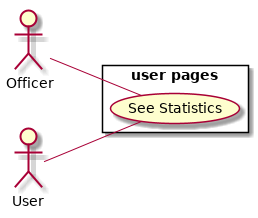
\includegraphics[width=\textwidth]{images/useCases/uc_statistics.png}
	\caption{Simple use case demonstrating the functionalities of SafeStreets application to provide statistics of its usage.} 
	\label{fig:statisticsuc} 
\end{figure}

\newpage
\begin{enumerate}
	\setcounter{enumi}{9}
	\item \textbf{Statistics and analytics consulting}\\
	\begin{table}[!htbp]
	\hypertarget{tab:statisticsconsultingtab}{}
	\centering
	\begin{tabular}{lp{9cm}}
		\bf\large Name&\bf\large Statistics and analytics consulting\\
		\hline
		\hline
		\bf Actors&Both Users or Officers\\
		\hline
		\bf Entry conditions&The actor is logged in and he is in the main page.\\
		\hline
		\bf Flow of events&
		\begin{itemize}
			
			\item The actor clicks on the "Statistics" button and is redirected to the page with alle the general SafeStreets statistics such as Tickets given, App usages, Effectiveness, Violation Types...
			
			\item The user clicks on the statistic he's interested in.
			
			\item The user could analyze the analytics provided and can compare different analytics to acquire knowledge about the SafeStreets project.
			
			\item After he finishes, he presses the Home button.
			
			\item The actor is then redirected to the main page.
			
		\end{itemize}
		\\
		\hline
		\bf Exit conditions&The actor-requested analytics is displayed to the user (these kind of information is not sensitive).\\
		\hline
		\bf Exceptions&None.
		\\
		\hline
		
	\end{tabular}
	\caption{Statistics consulting Use Case table}
	\label{tab:statisticsconsultingtab}
\end{table}
	\newpage
	\textbf{Diagrams}
	\usecasefiguresmall{general_statistics}{for an actor examining statistics}
	\newpage
\end{enumerate}
\newpage


	\subsection{Non functional requirements}
	\subsubsection{Performance}
    The application should be able to deliver the violations (including the
    \hyperref[sec:automatic_tickets]{automatic tickets}) in an acceptable time,
    which means at most 15 seconds, but should average to about 5 seconds.
    This is not a strict requirement, but it improves a lot the user experience and the possibility
    that he does not decide to give up with the upload.

    The 
    \hyperref[sec:data_mining]{data mining} 
    functionality is not as trivial as the delivery of the violations, but keeping in 
    mind the effectiveness of the user experience it should still be able to deliver results with an
    average waiting time of 5-10 seconds, with an upper bound of 20 seconds.

    The
    \hyperref[sec:request_for_interventions]{request for interventions}
    functionality does not have any time constraints, it should just end. It can be run at any time and
    its results will be stored on persistent storage, without the need to be used immediately.
    This functionality does however consume a lot of computer resources, since it must cross a large quantity
    of data from different sources and it will also use an AI. For this reason, it will have to run
    either when the load on the system is low or on a completely separate hardware.

    All the other operations that require an internet connection (login, logout...) should be fast enough
    to not become frustrating for the user to use the application, indicatively they should take 5 seconds at most.
    
\subsubsection{Reliability}
	As the system stores very important data, it must be ensured	that it is highly reliable and fault tolerant. For example, the	central	server,	which contains all the information, should be duplicated.\\The running processes (which provide the automatic ticket functionality) should be trustworthy, so if something goes wrong with an automatic ticket, that report that was generating the ticket should be put in a queue waiting that will be manually analyzed. In this way there must be ensured the consistency of information.\\Any other technique can be	adopted	to	ensure	the	required reliability.
    
\subsubsection{Availability}
	The system has no reasons to be highly available except for providing a great
user experience. So, since this is not a critical application, short period of
down could be acceptable.\\
	So, as SafeStreet does not need to be up to ensure critical aspects, but still some violations could have only a short period of time to be checked, it will have to guarantee a 99.9\% availability (43 minutes of downtime every month).

\subsubsection{Security}
    Since users will be able to give tickets automatically, security is a key aspect of the application.
    The information contained in the report of a violation must never be altered, and the login information
    must be kept safe to prevent hackers from giving false tickets using stolen identities.\\
    A public key encryption mechanism could be put in place to crypt reports when received by SafeStreets and to decrypt them only when the Police server has received them. As an alternative, the reports could be digitally signed with a trusted key of SafeStreets property.\\
  	Users also give their personal data when registering, and their privacy must be guaranteed. Techniques such as data encryption could be used to archive this.

\subsubsection{Scalability}
    This application will be a pioneer in this field, so it is difficult to foresee how many users will
    use it and how. A high degree of scalability is therefore required. To handle the first city,
    the system must handle 1 million registered users and a peak of 7.000 concurrent requests.
    
\subsubsection{Maintainability}
	An easy	to	fix	code, modify or update is preferable because,	according	to	the	circumstances it could be updated. That action should be done without too much pain and with a cheap cost.		
	Appropriate	design	patterns	will	be	used,	as	it	will	be	better	explained	in	a	further	document.    
	
\subsubsection{Portability}
	The application has to be compatible with the majority of devices present on the market in the last years, in order to
	increase the people eligible to become users of SafeStreets.
	
\subsubsection{Simple User Interface}
	The user interface has to be as simple and
	intuitive as possible, the application should allow an average user to set up
	an account and start using the application understanding its functionality
	in no more than a dozen minutes.
	
\subsubsection{Accuracy}
    The maximum error that the GPS system should commit for the application to accept a position is 15 meters,
    to let an eventual officer near the violation find the car.


	\clearpage
	\section{Formal Analysis using Alloy}
	This section employs the Alloy formal notation to provide a description of the domain,
the properties and the constraint of the model and to prove that they can be satisfied by the system.
	\subsection{Code}
	% alloy.sty
% Alloy mode for the LaTeX listings package.
% This is public domain

\definecolor{codegreen}{rgb}{0,0.6,0}
\definecolor{codegray}{rgb}{0.5,0.5,0.5}
\definecolor{codepurple}{rgb}{0.58,0,0.82}
\definecolor{backcolour}{rgb}{0.95,0.95,0.92}

\lstdefinelanguage{alloy}{
  keywords={%
      assert, pred, all, no, lone, one, some, check, run,
      but, let, implies, not, iff, in, and, or, set, sig, Int, int,
      if, then, else, exactly, disj, fact, fun, module, abstract,
      extends, open, none, univ, iden, seq,
  },
  literate=%
    {:}{$\colon$}1
    %{|}{$\pipe$}1
    {==}{$=$}1
    {=}{$=$}1
    {!=}{$\neq$}1
    {&&}{$\land$}1
    {||}{$\lor$}1
    {<=}{$\le$}1
    {>=}{$\ge$}1
    {all}{$\forall$}1
    {exists}{$\exists$}1
    {!in}{$\not\in$}1
    {\\in}{$\in$}1
    {=>}{$\implies$}2
    % the following isn't actually Alloy, but it gives the option to produce nicer latex
    {|=>}{$\Rightarrow$}2
    {<=set}{$\subseteq$}1
    {+set}{$\cup$}1
    {*set}{$\cap$}1
    {==>}{$\Longrightarrow$}3
    {<==>}{$\Longleftrightarrow$}4
    {...}{$\ldots$}1
    {\\hl}{$\hline$}1
    {\\alpha}{$\alpha$}1
    {\\beta}{$\beta$}1
    {\\gamma}{$\gamma$}1
    {\\delta}{$\delta$}1
    {\\epsilon}{$\epsilon$}1
    {\\zeta}{$\zeta$}1
    {\\eta}{$\eta$}1
    {\\theta}{$\theta$}1
    {\\iota}{$\iota$}1
    {\\kappa}{$\kappa$}1
    {\\lambda}{$\lambda$}1
    {\\mu}{$\mu$}1
    {\\nu}{$\nu$}1
    {\\xi}{$\xi$}1
    {\\pi}{$\pi$}1
    {\\rho}{$\rho$}1
    {\\sigma}{$\sigma$}1
    {\\tau}{$\tau$}1
    {\\upsilon}{$\upsilon$}1
    {\\phi}{$\phi$}1
    {\\chi}{$\chi$}1
    {\\psi}{$\psi$}1
    {\\omega}{$\omega$}1
    {\\Gamma}{$\Gamma$}1
    {\\Delta}{$\Delta$}1
    {\\Theta}{$\Theta$}1
    {\\Lambda}{$\Lambda$}1
    {\\Xi}{$\Xi$}1
    {\\Pi}{$\Pi$}1
    {\\Sigma}{$\Sigma$}1
    {\\Upsilon}{$\Upsilon$}1
    {\\Phi}{$\Phi$}1
    {\\Psi}{$\Psi$}1
    {\\Omega}{$\Omega$}1
    {\\EOF}{\;}1
    ,
  sensitive=true,  % case sensitive
  morecomment=[l]//,%
  morecomment=[l]{--},%
  morecomment=[s]{/*}{*/},%
  morestring=[b]",
  firstnumber=1,
  numberstyle=\tiny\color{codegray},
  basicstyle=\scriptsize\ttfamily,
  commentstyle=\itshape\color{codegreen},
  keywordstyle=\bfseries\color{codepurple},
  ndkeywordstyle=\bfseries,
  numbers=left,
  numbersep=5pt,
  tabsize=2,
  breaklines=true,
  %postbreak=\mbox{\textcolor{red}{$\hookrightarrow$}\space}
}

% inline
\def\A{%
    \lstinline[language=alloy,basicstyle=\ttfamily,columns=fixed]}

% paragraph
\lstnewenvironment{alloy}[1][]{%
  \lstset{language=alloy,
    floatplacement={tbp},captionpos=b,
    xleftmargin=8pt,xrightmargin=8pt,basicstyle=\ttfamily,#1}}{}

% paragraph from file
\newcommand{\alloyfile}[1]{
  \lstinputlisting[language=alloy,%
    frame=lines,xleftmargin=8pt,xrightmargin=8pt,basicstyle=\ttfamily,columns=fixed]{#1}
}

\alloyfile{alloy/safeStreets.als}
	
	\clearpage
	\section{Softwares Used and Effort Spent}
	\subsection{Softwares Used}
	\begin{flushleft}

\begin{table}[htp]
	\centering

\begin{tabular}{|c|c|}
\hline
Task&Software Used\\
\hline
Edit and compile LATEX code&TeXstudio and VisualStudioCode\\
\hline
UML modelling&-\\
\hline
Run and compile Alloy&-\\
\hline
Mockup&Moqups\\
\hline

\end{tabular}

\caption{Softwares used} 

\end{table}

\end{flushleft}
	\subsection{Effort Spent}
		
	\begin{table}[htp]
		\centering
		\begin{tabular}{|c|c|}
			\hline
			Student&Hours spent\\
			\hline
			Andrea Furlan&-\\
			\hline
			Cosimo Russo&-\\
			\hline
			Giorgio Ughini&-\\
			\hline
			
		\end{tabular}
		
		\caption{Effort spent} 
		
	\end{table}




\end{document}